The following section describes the procedure used to select the events used for analysis. First, the data and simulation samples to be used are defined. Then, the fiducial definition of the physics objects used to select the events is given. Then, the criteria for selecting events is discussed. Finally, the event yields and reconstructed distributions are reviewed.

\section{Data samples}
Data and Monte Carlo samples are used in the common D3PD format ({\texttt NTUP\_COMMON}), using the {\texttt p1562} processing tag. The D3PDs are processed using software based on {\texttt AnalysisTop-1.8.0}~\cite{trc}.

\subsection{Collision data}
The analysis is performed on the complete 2012 $pp$  \rts=8 \tev\ LHC collision dataset. Events are required to
fulfill standard data quality requirements corresponding to the physics  `AllGood' good run list (GRL)~\cite{grl}, which ensures that all detector components are functioning. Events are required to pass a single electron or single muon trigger chain, with thresholds that are maximally efficient for leptons passing offline selections of $p_T>25$\,GeV.  For electrons, the OR of the {\texttt EF\_24vh\_medium1}\ and {\texttt EF\_e60\_medium1}\ trigger chains is used. For muons, the OR of {\texttt EF\_mu24i\_tight}\ and {\texttt EF\_mu36\_tight} is used. In each case, the higher threshold trigger has no isolation requirement, and adds to the acceptance of the lower threshold trigger at higher lepton $p_T$. 

Events are selected from both {\texttt Egamma} and {\texttt Muons} data streams. To avoid double counting of $e\mu$ events appearing in both streams, events passing electron triggers are only accepted from the {\texttt Egamma} stream, {\em i.e.} the {\texttt Muons} stream is only used for events selected {\emph only} by muon triggers. Luminosity blocks where only one stream is seen in the final analysis are vetoed, to avoid biases from losing events from either stream in the upstream reconstruction and data processing. 
After all these selections, the final analyzed data samples correspond to an integrated luminosity of 20.3\,\ifb\ with an uncertainty of 2.8\%.
\subsection{Simulated Samples}

Simulated Monte Carlo event samples are used in this analysis to evaluate the efficiency and uncertainty of signal and background.  Both uncorrected and corrected data distributions are also compared to simulated samples to distiguish between physics models. 
Standard ATLAS top group MC12 samples are used.~\cite{topmc} The corresponding dataset (DS) identification numbers are given  in Tables~\ref{t:ttsamples},~\ref{t:bgsamples}, and ~\ref{t:wtsamples} and a complete list of dataset names is provided in Appendix~\ref{app:ds}.

Samples are processed either through the full ATLAS Geant4\cite{bib:g4} based detector simulation or through the {\texttt AtlFast2}\cite{atlfast2} fast simulation. All samples include additional overlaid minimum bias events generated with {\textsc  Pythia8} \cite{pythia8} to simulate pileup background. 
The simulated samples are reweighted to reproduce the same distributions of $\mu$, the average number of interactions per bunch crossing, as the data. The samples are also reweighted with scale factors to reproduce the electron and muon reconstruction and trigger efficiencies, and the width of the primary vertex distribution in $z$, as measured in the data. Finally, scale factors are applied to account for $b$-tagging efficiencies.  In all cases,
the scale factors are those specificed in {\texttt AnalysisTop-1.8.0}.

All Monte Carlo samples are normalized according to the best available theoretical cross-section and $K$-factor calculations, as tabulated in the {\texttt TopDataPreparation} package, tag {\texttt 00-06-48}.

\subsubsection{\ttbar samples}\label{ss:mcsignal}

The baseline \ttbar\ samples are produced using {\textsc  Powheg} \cite{Powheg, Powheg2, Powheg3, Powheg4} interfaced to {\textsc  Pythia6} \cite{pythia6} with the Perugia 2011C tune \cite{perugia}, CT10 parton density functions (PDFs) \cite{cttenpdf}, the hdamp parameter set to $\infty$ and fast simulation (DS 117050).  
This same MC tune has been processed using full simulation and the results of the two samples have been compared.
%After appropriate
%JES corrections are applied, systematic differences in the prediction are observed. 
%The stress test in Section~\ref{sec:unfold} confirms the agreement of these two samples.
{\textsc  Powheg}+{\textsc  Pythia6} is the baseline suggested by the TopReconstruction twiki page as the default \ttbar\ simulation~\cite{topmc}. The atlfast2 sample with the hdamp parameter set to $\infty$ is chosen as the baseline because it has signifigantly higher statistics ($\sim 40$ times data) than either the FS or hdamp=$m_t$ samples ($\sim 20$ times data).
Systematic uncertainties associated with the difference in the response matrices obtained from FS and atlfast are
assessed in Section~\ref{sec:syst}.


%For the baseline dataset, samples using both full and fast  simulation are analyzed to confirm that after making appropriate JES corrections, there are no differences in the predictions.

Alternative \ttbar\ simulation samples are also studied.  At next-to-leading-order, these include {\textsc  Powheg} plus {\textsc  Pythia6}  with the hdamp parameter set to $m_{t}$ (DS 110404); {\textsc  Powheg} plus {\textsc  Pythia8} with the hdamp parameter set to $m_{t}$ and the A14 tune (DS117046) ; {\textsc  MC@NLO} \cite{mcatnlo, mcatnlo2} interfaced to {\textsc  Herwig} \cite{Herwig, Herwig1, Herwig2} with {\textsc  Jimmy} \cite{jimmy} for the underlying event modeling and with the ATLAS AUET2 \cite{auet} tune and CT10 PDFs (DS 105200); and {\textsc  Powheg} plus {\textsc  Herwig} (DS 105860). 
Alternate multi-leg leading order samples include {\textsc  MadGraph} \cite{Alwall:2011uj} interfaced to {\textsc  Pythia6} \cite{pythia6} with the Perugia 2011C tune \cite{perugia}, and CT10 parton density functions (PDFs) \cite{cttenpdf} (DS 110872); {\textsc  Alpgen} \cite{alpgen} interfaced to {\textsc  Herwig} and {\textsc  Jimmy}, with
the CTEQ6L1 PDFs \cite{CTEQ} (DS 105890--2, 117897--9, 116108 and 116109); and {\textsc  Alpgen} interfaced to {\textsc  Pythia6}
(DS 117113--8). To study the effects of initial and final state radiation (ISR/FSR), several samples with different radition parameters were used.

%ADD IN HERWIG FOR PARTON SHOWERING+MADGRAPH Q2+ISR FSR

The {\textsc  Powheg} and {\textsc  MC@NLO} samples include all \ttbar\ final states except fully-hadronic, where both $W$ bosons decay to \qqbar\ giving a negligible probability to pass the event selection. The {\textsc  MadGraph} sample only included dileptonic final states, where both $W$ bosons decay to leptons. Most of these MC samples contain more than ten times the data statistics.

\subsubsection{Single top samples}
Only the $Wt$ channel of single top production contributes significantly to \emubb\ events. Single top production is modeled using {\textsc  Powheg+Pythia} with the CT10 PDFs and the Perugia P2011C tune, using the `diagram removal' \cite{Frixione:2008yi} generation scheme (DS 110140). Alternative physics models include the {\textsc  Powheg+Pythia} sample with `diagram subtraction' \cite{Frixione:2008yi} (DS 110142) and \mcnlohw (DS 108346).

\subsubsection{Background samples}\label{ss:mcbkg}

$Z$+jets events with $Z\rightarrow \ell^-\ell^+$ and diboson production ($WW$, $WZ$ and~$ZZ$) where both bosons decay leptonically can contribute to background. $Z$+jets background is modeled using {\textsc  Alpgen} \cite{Mangano:2002ea} with CTEQ6L1 PDFs, interfaced to {\textsc  Pythia6} with the Perugia P2011C tune, including both samples with 0--5 additional light partons (DS 147105--10, 147113--8, 147121--6), 
\ccbar\ plus an additional 0--3 partons (DS 200432--5, 200440--3, 200448--51), and \bbbar\
plus 0--3 partons (DS 200332--5, 200340--3, 200348--51). The heavy flavor overlap procedure (HFOR) \cite{hfor} is used to avoid double counting of configurations where the \ccbar\ or \bbbar\ pair could be produced from either the matrix element or parton shower. The simulated $Z+$jets  events are scaled by the ratios of $Z\rarrow ee$+2 $b$-jets or $Z\rarrow \mu\mu$+2 $b$-jets measured in simulation and data, to account for the mismodeling of heavy-flavor jets produced with $Z$ bosons. Ref.~\cite{xsec} computes this scale factor to be $1.13 \pm 0.08$. 

Diboson production is simulated using {\textsc  Alpgen+Herwig} with up to three additional partons (DS 107100--11).


\begin{table}
{\small
\begin{tabular}{|lc|l|l|l|l|}\hline
Generator & Dataset & Sim & FS & Tune  & Comment \\ \hline
{\textsc  Powheg+Pythia} hdamp=$\infty$ & 117050 & fast & nFH & P2011C &  baseline\\
\hline
{\textsc  Powheg+Pythia} hdamp=$m_t$ & 110404 & fast & nFH & P2011C &  alt. physics \\
{\textsc  MC@NLO+Herwig} & 105200 & fast & nFH & P2011C & alt. physics \\
{\textsc  Powheg+Herwig} & 105860 & fast & nFH & AUET2 & alt. shower \\
{\textsc  Powheg+Pythia8} & 117046 & fast & nFH & A14 & alt. physics \\
\hline
{\textsc  MadGraph+Pythia} & 110872 & fast & $\ell\ell$ & P2011C & alt. physics \\
{\textsc  Alpgen+Pythia} & 201020-4 & fast & nFH & P2012 & alt. physics \\
{\textsc  Alpgen+Herwig} & 164440-3, & full & nFH  & P2012 & alt. physics \\
{\textsc  Alpgen+Herwig} & 116108 & full & nFH & P2012 & alt. physics \\
{\textsc  Alpgen+Herwig} & 116109 & full & nFH & P2012 & alt. physics \\
\hline
{\textsc  AcerMC+Pythia} & 117209 &  fast & nFH & MPS AUET2 & more radiation \\
{\textsc  AcerMC+Pythia} & 117210 &  fast & nFH & LPS AUET2 & less radiation \\
{\textsc  Alpgen+Pythia} & 201030-4 & fast & nFH & P2012 & ktfac=0.5, more radiation tune \\
{\textsc  Alpgen+Pythia} & 201040-4 & fast & nFH & P2012 & ktfac=2, less radiation tune \\
{\textsc  MadGraph+Pythia} & 110878 & fast & $\ell\ell$ & P2011C & more radiation tune \\
{\textsc  MadGraph+Pythia} & 110875 & fast & $\ell\ell$ & P2011C & less radiation tune \\
\hline \hline
\end{tabular}
}
\caption{\ttbar samples used in this
analysis. The sample name, dataset ID, simulation type, final state simulated 
(non-fully hadronic, nFH, or dilepton, $\ell\ell$) and tune is given. The {\textsc  Alpgen} samples consist of several samples
with different parton multiplicities and sometimes dedicated heavy flavor samples.\label{t:ttsamples}}
\end{table}


\begin{table}
\begin{center}
\begin{tabular}{|lc|l|l|l|l|}\hline
Generator &  Process  & Sim  & FS & Tune  & Comment \\ \hline

{\textsc  Alpgen+Herwig } & Diboson  & full & $\ell\ell$  & AUET2 &  \\
{\textsc  Alpgen+Pythia }  & $Z$+jets  &  full &  $\ell\ell$ & P2011C &   On-the-fly \\
\hline \hline
\end{tabular}
\end{center}
\caption{$Z$+jets and diboson background samples used in this
analysis. The sample name, process, simulation type, process simulated, final state simulated 
(non-fully hadronic, nFH, or dilepton, $\ell\ell$) and tune is given. The {\textsc  Alpgen} samples consist of several samples
with different parton multiplicities and sometimes dedicated heavy flavor samples. Dataset IDs are listed in Appendix~\ref{app:ds}.\label{t:bgsamples}}
\end{table}

\begin{table}
\begin{center}
\begin{tabular}{|lc|l|l|l|}\hline
Generator & Dataset & Sim & Tune  & Comment \\ \hline
{\textsc  Powheg+Pythia} & 110140 & fast & P2011C & baseline diagram removal \\
\hline
{\textsc  Powheg+Pythia} & 110142 & full & P2011C & alt. diagram subtraction \\
\mcnlohw & 108346 & full   & AUET2 & alt. physics \\
\hline \hline
\end{tabular}
\caption{Single top $Wt$-channel samples used in this
analysis. The sample name, dataset ID, simulation type, and tune is given. All samples are simulated with the inclusive final state in the $Wt$ channel.\label{t:wtsamples}}
\end{center}
\end{table}

%\begin{table}
%\begin{center}
%\begin{tabular}{|lc|l|l|l|l|}\hline
%Generator &  Process  & Sim  & FS & Tune  & Comment \\ \hline
%\hline \hline
%\end{tabular}
%\begin{center}
%\caption{Evgen samples to be added here (if/when used)\label{t:evgen}}
%\end{table}
%\end{center}
\subsection{Pileup jet samples}
Samples using pileup overlay simulation in \ttbar\ events are used to study background to the extra jet distributions. The only sample with sufficient statistics (DS 117050) uses {\textsc  Powheg+Pythia} with the baseline tune. The sample was processed using tag {\texttt d708} which is affected by a simulation problem in the tile cell energy. An additional sample has been requested, but production is delayed by problems with ProdSys2.\footnote{JIRA entry {\textsc  ATLMCPROD-821}} 

Because of limitations with the available overlay samples, a data driven estimate of the pileup is used for the baseline
analysis.  This estimate uses 
data from the {\texttt data12\_8TeV.physics\_ZeroBiasOverlay}, which are events taken from data to estimate pileup. These data are available in {\texttt NTUP\_COMMON} format. This sample is studied as an alternative to the standard minimum bias overlay in the other samples.
\section{Object definitions}
The object and event selection follows the generic ATLAS top working
group recommendations for 2012 \cite{topreco}, with two exceptions. The first change is a loosening of the electron isolation criteria, which is possible due to the low background  $e\mu$ final state. This loosened requirement is also used in Ref.~\cite{xsec}. The second change is to relax the $\eta$ requirement on  jets to $|\eta|<4.5$.

\subsection{Reconstructed objects}\label{s:objects}

The analysis relies on the selection of electrons, muons and jets, and
the tagging of jets as $b$-jets. With the exceptions specified above, these correspond to standard {\texttt TopRootCore} defaults.
\begin{description}
\item[Muons:] Combined muons (reconstructed in both the muon spectrometer
and inner detector) are selected with the {\texttt MuID} algorithm, and 
required to satisfy $p_T>25$\,GeV and $|\eta|<2.5$.  Following the 2012 recommendations from the MuonCP group, muons must have
\begin{itemize}
\item at least one pixel hit
\item at least 5 SCT hits
\item fewer than 3 holes in pixel and SCT layers combined
\item In the region $0.1 < |\eta| < 1.9 $: $n_{TRT Hits} + n_{TRT Outliers} > 5$ and $\frac{n_{TRT Hits}}{n_{TRT Hits} + n_{TRT Outliers}} < 0.9$
\end{itemize}

The impact parameter
in the longitudinal direction with respect to the primary vertex is
required to satisfy $z_0<2$\,mm.  To reduce the background from
muons from heavy flavor decays inside jets, muons are required to be
separated by $\Delta R>0.4$ from the nearest jet. Muons are required to satisfy 
mini-isolation requirement $I^\ell_{\textrm mini}<0.05$, where
the mini-isolation variable is the ratio of the sum of $p_T$ of tracks
in a variable-sized cone of radius $\Delta R=10\,{\textrm GeV}/p_T(\mu)$ to the $p_T$ of the muon $p_T(\mu)$ \cite{topreco}. %For anti-muons, the mini-isolation requirement is energy loss of less than 6 GeV, ${\texttt ETCone20}/p_{T} < 0.03$, and $I^\ell_{\textrm mini}<0.1$

\item[Electrons:] Electrons are selected using the offline {\texttt tight++} 
identification within the fiducial region $p_T>25$\,GeV and $|\eta|<2.47$, 
excluding the calorimeter transition region $1.37<|\eta|<1.52$. The impact parameter
in the longitudinal direction with respect to the primary vertex is
required to satisfy $z_0<2$\,mm. In addition 
to the calorimeter isolation requirements implicit in {\texttt tight++},
the calorimeter energy in a cone of radius $\Delta R<0.2$ around the
electron (excluding the deposit from the electron itself) is required
to satisfy ${\texttt ETCone20}<6$\,GeV, and the sum of $p_T$ of tracks
in a cone of radius $\Delta R<0.3$ (excluding the electron track) is
required to satisfy ${\texttt pTCone30}<6$\,GeV. Using the
EGamma group {\texttt EisoTool2012} \cite{eisotool}, further
kinematic-dependent cuts are applied to these two isolation variables,
corresponding to a 98\,\% efficiency on true prompt electrons. 
To prevent double-counting
of electron energy deposits as jets, jets within $\Delta R<0.2$ of 
a reconstructed electron are removed. If the nearest jet surviving
the above cut is within $\Delta R<0.4$ of the electron, the electron
is discarded, to ensure it is cleanly separated from nearby jet activity. Electrons sharing a track with a muon are excluded by removing electrons with a muon within $\Delta \phi < 0.005$ and $\Delta \theta < 0.005$.

\item[Jets:] Jets are reconstructed using the anti-$k_t$ algorithm 
\cite{antikt} with radius parameter $R=0.4$, 
starting from topological clusters. These are calibrated
using the local cluster weighting (LCW) method, and corrected for the
effects of pileup using the jet area method and a residual correction dependent
on the instantaneous luminosity and number of reconstructed primary vertices 
in the event. Jets are calibrated using an energy- and $\eta$-dependent simulation-based calibration scheme, with in-situ corrections 
based on data \cite{jesxi}. Jets are accepted within the fiducial region $p_T>25$\,GeV and $|\eta|<4.5$. To reduce the contribution from jets 
associated with pileup jets with $p_T<50$\,GeV
are required to satisfy $|\textrm JVF|>0.5$, where $\textrm JVF$ is
the ratio of the sum of the $p_T$ of tracks associated to the jet which
are also associated to the primary vertex, to the sum of $p_T$ of all
tracks associated to the jet. Jets with no associated tracks or with
$|\eta|>2.4$ at the edge of the tracker acceptance  are assigned
$\textrm JVF=-1$ by convention and thus always accepted.
Reconstructed jets 
within $\Delta R<0.2$ of a selected electron are removed.

\item[$b$-tagging:] Jets within the central region ($|\eta| < 2.5$) are $b$-tagged using the MV1 algorithm 
\cite{btagcom,btagptrel},
which combines the outputs of the IP3D, SV1 and JetFitterCombNN algorithms
into a multivariate discriminant $w$ with values between zero and one. 
Light-quark and gluon jets tend to have values close to zero, and 
$b$-flavored jets close to one, with charm jets somewhere in between. Jets are defined as being $b$-tagged if the MV1 weight $w$ is larger than a cut value 0.7892, which corresponds to the $b$-tagging working 
point having approximately 70\% $b$-tagging efficiency for $b$-jets in \ttbar\ events, although the exact efficiency varies significantly with $p_T$. The $b$-tagging calibration used is the default in {\texttt TopRootCore}, which is based on the system8 muon and jet calibration method~\cite{btagsys8}.
\end{description}
Events reconstructed with exactly one $e$ and $\mu$ with opposite sign and at least 2-$b$ jets as defined above pass the reconstruction-level fiducial selection. In the case of Monte Carlo, selected events are reweighted to reproduce the same distributions of $\mu$, the average number of interactions per bunch crossing, as in the data. The samples are also reweighted with scale factors to reproduce the electron and muon reconstruction and trigger efficiencies, and the width of the primary vertex distribution in $z$, as measured in the data. Finally, scale factors are applied to account for $b$-tagging efficiencies.
\subsection{Truth objects}
Truth objects are processed using the software package {\texttt TopFiducial-00-00-09} in {\texttt AnalysisTop-1.8.0}. Cuts applied to truth objects attempt to replicate the above fiducial selections for the reconstructed objects.

\begin{description}
\item[Leptons:] Stable electrons and muons are required not to come from a hadron in the Monte Carlo truth particle record, either directly or through a tau decay. This ensures that the lepton is from an electroweak decay without requiring a direct $W$-boson match. The four momenta of the bare leptons are then `dressed' by adding the four momenta of all stable photons within $\Delta R$=0.1 with status code 1 and not originating from Geant4. The dressed leptons are required to have \pt > 25 \GeV\ and $|\eta|$ < 2.5.
\item[Jets:] Truth jets are clustered using the anti-$k_t$ algorithm \cite{antikt} with radius parameter $R=0.4$, starting from all stable particles, except for selected leptons ($e$, $\mu$, $\nu$) and the photons used to dress the leptons. Truth jets are required to have \pT > 10 \GeV, $|\eta|$ < 4.5. Though only jets with \pT > 25 \GeV\ are considered in the final result, lowering the \pt\ requirement for truth jets allows matching across the fiducial boundary. This is discussed in more detail in Section~\ref{sec:extrajets}.

\item[$b$-tagging:] $B$ hadrons with \pT > 5 \GeV\ are associated with jets through ghost matching~\cite{ghostmatch}. Truth $b$-tagged jets have \pT > 25 \GeV, $|\eta|$ < 2.5 and at least one ghost associated $B$-hadron with $p^{{\textrm B}}_{T} > 5$ \GeV.

\item[Overlap removal:] Truth objects are subject to the same overlap removal criteria as reconstructed objects, after dressing and jet reclustering. The closest jet within $\Delta R$ < 0.2 of an electron is excluded from consideration.  After such jets are removed, 
muons  and electrons with $\Delta R$ < 0.4 of a jet are excluded. Electrons overlapping with muons are removed if $\Delta \phi_{e\mu} < 0.005$ and $\Delta \theta_{e\mu} < 0.005$.
\end{description}


Events with exactly one $e$ and $\mu$ with opposite sign and at least 2-$b$ jets as defined above pass the fiducial truth selection.

\subsection{Truth matching}
\label{ss:tmatching}
Following {\texttt TopFiducial} standard criteria, a geometric $\Delta R$ algorithm matches reconstructed objects to truth objects satisfying the fiducial requirements above. These definitions are relevant for background unmatched extra jets, as well as various truth studies.
\begin{description}
\item[Leptons:] Each truth $e$ ($\mu$) is matched to the closest reconstructed $e$ ($\mu$) within $\Delta R < 0.02$.
\item[Jets:] Truth jets are geometrically matched to the closest reconstructed jet within $\Delta R_{\mathrm{reco jet, truth jet}} < 0.4$. If a reconstructed jet is not matched to a truth jet, it is assumed to be either from pileup or matching inefficiency and is treated as background as discussed in Section~\ref{ss:pileup}.

In selecting $e\mu$+2 $b$-jet events, $b$-jets are matched to truth jets before extra jets. Thus, if both an extra jet and a $b$-jet satisfy $\Delta R_{\mathrm{reco jet, truth jet}}<0.4$, the $b$-jet is matched to the truth jet and the extra jet is unmatched. If two $b$-jets or two extra jets are reconstructed within $\Delta R_{\mathrm{reco jet, truth jet}}<0.4$ of a single truth jet, the reconstructed jet with smaller $\Delta R_{\mathrm{reco jet, truth jet}}$ is matched to the truth jet and the other reconstructed jet is unmatched.

Because of limited \pt\ resolution, the reconstructed \pt\ of a jet can vary significantly from its truth \pt. The \pt\ threshold for truth jets is lowered to 10 \GeV, so that jets reconstructed with \pt\ > 25 \GeV\ can match truth jets that fail the fiducial \pt\ cut. 



\item[Parton matching:] For some studies, the truth jets from top are identified via a parton matching procedure. Each jet is matched to the highest energy parton\footnote{Quarks (u,d,s,c,b), gluons, photons and pdgId = 0 particles.} with \pt > 5 \GeV\ within $\Delta R = 0.4$. If this parton is a decay product of the top, then the jet is considered a `top jet.'
\end{description}
\section{Event selection}
The process of selecting \emubb\ events proceeds as follows. First, events are selected from simulation and data by vetoing a small number of events failing cleaning cuts. Then events are required to have exactly one electron and one muon with opposite charges. Finally, events with at least two $b$-tagged jets are selected. In events with more than two $b$-tagged jets, the two $b$-jets with the highest MV1 are considered the $b$-jets used to select the event and the remaining $b$-jet(s) are considered extra jets. The selection requirements are identical to those in the 2012 \ttbar cross-section analysis~\cite{xsec}, with the exception of requiring \textit{at least} two $b$-tagged jets instead of \textit{exactly} two.

\subsection{Cleaning cuts}

Events are required to have at least one reconstructed primary vertex with at least five associated tracks. Events containing any jets with $p_T>20\GeV$ and positive energy that fail the `Bad Loose Minus' (also known as  `Looser') jet quality cuts \cite{jetcleaning} are removed (`jet cleaning'). To remove events containing cosmic rays, events with two muons passing the muon selection requirements given above, each having an impact parameter with respect to the primary vertex $d_0>0.5$\,mm and separated in azimuthal angle $\phi$ by $\Delta\phi>3.1$\,rad, are vetoed.

A muon undergoing catastrophic bremsstrahlung/energy loss in the calorimeter
can leave a large energy deposit, causing it to be reconstructed as both
an electron and a muon, and potentially giving rise to a fake $e\mu$ event.  Such background is reduced by vetoing $e\mu$ events if the electron and muon are separated by $\Delta\phi<0.005$ and $\Delta\theta<0.005$, where $\phi$ and $\theta$ are the azimuthal and polar angles of the selected leptons
(muon bremsstrahlung cut).

\subsection{Event yields}

The numbers of events with exactly one $e$ and one $\mu$ before and after the $b$-jet requirement are given in Table~\ref{t:sel}. The events are selected from the 2012 \rts=8 \TeV data with 20.3 \ifb. Simulation predictions are categorized into contributions from \ttbar, $Wt$ single top, $Z$+jets and dibosons. 

After the selection of $e\mu$ opposite-sign pairs, the biggest contribution (60\%) is from \ttbar events with the second largest from $Z$+jets (21.8\%). The $e\mu$ event rates agree to  better than 3\% with those from other ongoing 2012 top analyses as documented in {\texttt TopEventChallenge}\cite{topeventchallenge}. The events with at least 2 $b$-jets are heavily dominated by \ttbar events, with a small $\sim 3\%$ contribution from single top. $Z$+jets and dibosons make up less than 0.1\% of events passing the final selection, and are thus neglected in this analysis.


The number of selected events in simulation and data agree to within better than 3\%, demonstrating that the Monte Carlo reproduces the data quite well. Table~\ref{t:ttgen} compares the number of selected events from the baseline \ttbar simulation to those from other \ttbar generators. The two \pow+\py\ simulations and \mcnlohw\ all agree with each other to within ~2\%. The \madpy\ simulation gives about 10\% more events. The reason for this difference is not well understood. The last column in Table~\ref{t:ttgen} gives the scale factor used to normalize each \ttbar generator to the number of events in data (including the single top contribution).

%To facilitate comparison with Ref.~\cite{xsecnote}, Table~\ref{t:exact2sel} gives the number of \ttbar simulation and data events with exactly 2 $b$-jets. Removing events with more than 2 $b$-jets reduces the number of events by ~2\% in both simulation and data. The event counts given in Table 4.2 of Ref.~\cite{xsecnote} are not directly comparable because they exclude contributions from misidentified leptons and correspond to a greater luminosity of 20.3\ifb. Adding back in the misidentified lepton contribution and then scaling by $20.1/20.3=0.989$ gives an `adjusted' event count in the final column. This analysis finds 2.1\% more events in data and 0.3\% more events in simulation than Ref.~\cite{xsecnote}. These differences are likely due to the new calibrations used in this analysis.


\subsection{Reconstructed distributions}
In Figures~\ref{fig:emu} and ~\ref{fig:bjet}, the properties of reconstructed lepton and $b$-jets in $e\mu$+2 $b$-jet events are compared in simulation and data. The negligible contributions from $Z$+jets and dibosons are not shown. Simulation is normalized to the number of events in data using the scale factors in Table~\ref{t:ttgen} in order to study the shape differences and remove uncertainties from the \ttbar cross section. In Figures~\ref{fig:emu} and ~\ref{fig:bjet}, the statistical uncertainity on the data is shown as a gray band on the ratio plot and statistical uncertainties on the simulation are shown as error bars on the ratio. Systematic uncertainities are not shown.

Figure~\ref{fig:emu} shows the \pt\ and $\eta$ distributions of the leptons. 
%The modeled \pt spectra are slightly softer than those in data. 
%The baseline \pow+\py hdamp=$\infty$ best reproduces the lepton $\eta$ observed in data. 
Figure~\ref{fig:bjet} shows the \pt\ and $\eta$ distributions of the 2 $b$-jets used to select the events. 
%\hdamp and \powpy\ agree best with the $b$-jet \pt in data, while the other three generators have slightly softer distributions. The $b$-jet $\eta$ is modeled well by all simulations.

Overall, the $b$-jets and the leptons are well modeled by simulation. \pow+\py\ hdamp=$\infty$ agrees  well, motivating its suitability as a baseline simulation.\footnote{The baseline sample is primarily chosen for high statistics} These observations are consistent with those in Ref.~\cite{xsecnote}.

\begin{table}[htp]
\centering
\begin{tabular}{|l|cc|cc|}\hline
Component & $e\mu$ & (\%) & $\geq$ 2-$b$ jets & (\%) \\ \hline
$t\bar{t}$ 	& 40542.1	& 59.4 	& 11946.5 &	97.1 \\
Single top 	& 3955.8	& 5.8	& 356.3 &	2.9 \\
Z+jets 		& 15117.4 	& 22.1	& 4.5 	&	0.0 \\
Dibosons 	& 8585.7 	& 12.6 	& 1.7	&	0.0 \\
\hline
Total & 68201.0 & 100.0 & 12309	& 100.0 \\
\hline
Data & 69575 &  & 12332 &   \\
\hline \hline 
\end{tabular}
\caption{Number of events with opposite sign $e\mu$ and at least 2 $b$-jets in the data  compared to that from Monte Carlo, broken down into contributions from \ttbar, $Wt$ single top, Z+jets and dibosons. Only central values are shown here;  systematic uncertainties are discussed in Section~\ref{sec:syst}.}
\label{t:sel}
\end{table}

\begin{table}[htp]
\begin{center}
\begin{tabular} {|l|l|l||l|}
\hline
Generator & DS & $N_{\ttbar}$ & $N_{\mathrm{data}}/(N_{\text{single~top}}+N_{\ttbar})$\\
\hline
\pow+\py hdamp=$\infty$ (base) & 117050 & 11946.5 & 1.0024\\
\pow+\py P2011C hdamp=$m_t$ & 110404 & 12095.8 & 0.9904 \\
\mcnlohw\ & 105200 & 12208.3 & 0.9815 \\
\madgraph+\py & 110872 & 356.33 & 0.9194 \\
\pow+\hw & 105860 & 11856.6 & 1.0097 \\
\peight & 117046 & 12115.6 & 0.9888 \\

\hline
\end{tabular}
\end{center}
\caption{Number of events with an opposite sign $e\mu$ and at least 2 $b$-jets for different \ttbar generators. The last column gives scale factor to normalize the sum of the \ttbar\ simulatation and single top yields ($N_{\mathrm{single~top}}=361.4$) to the data yield (12332).}
\label{t:ttgen}
\end{table}


\begin{figure}
\centering
\subfloat[]{
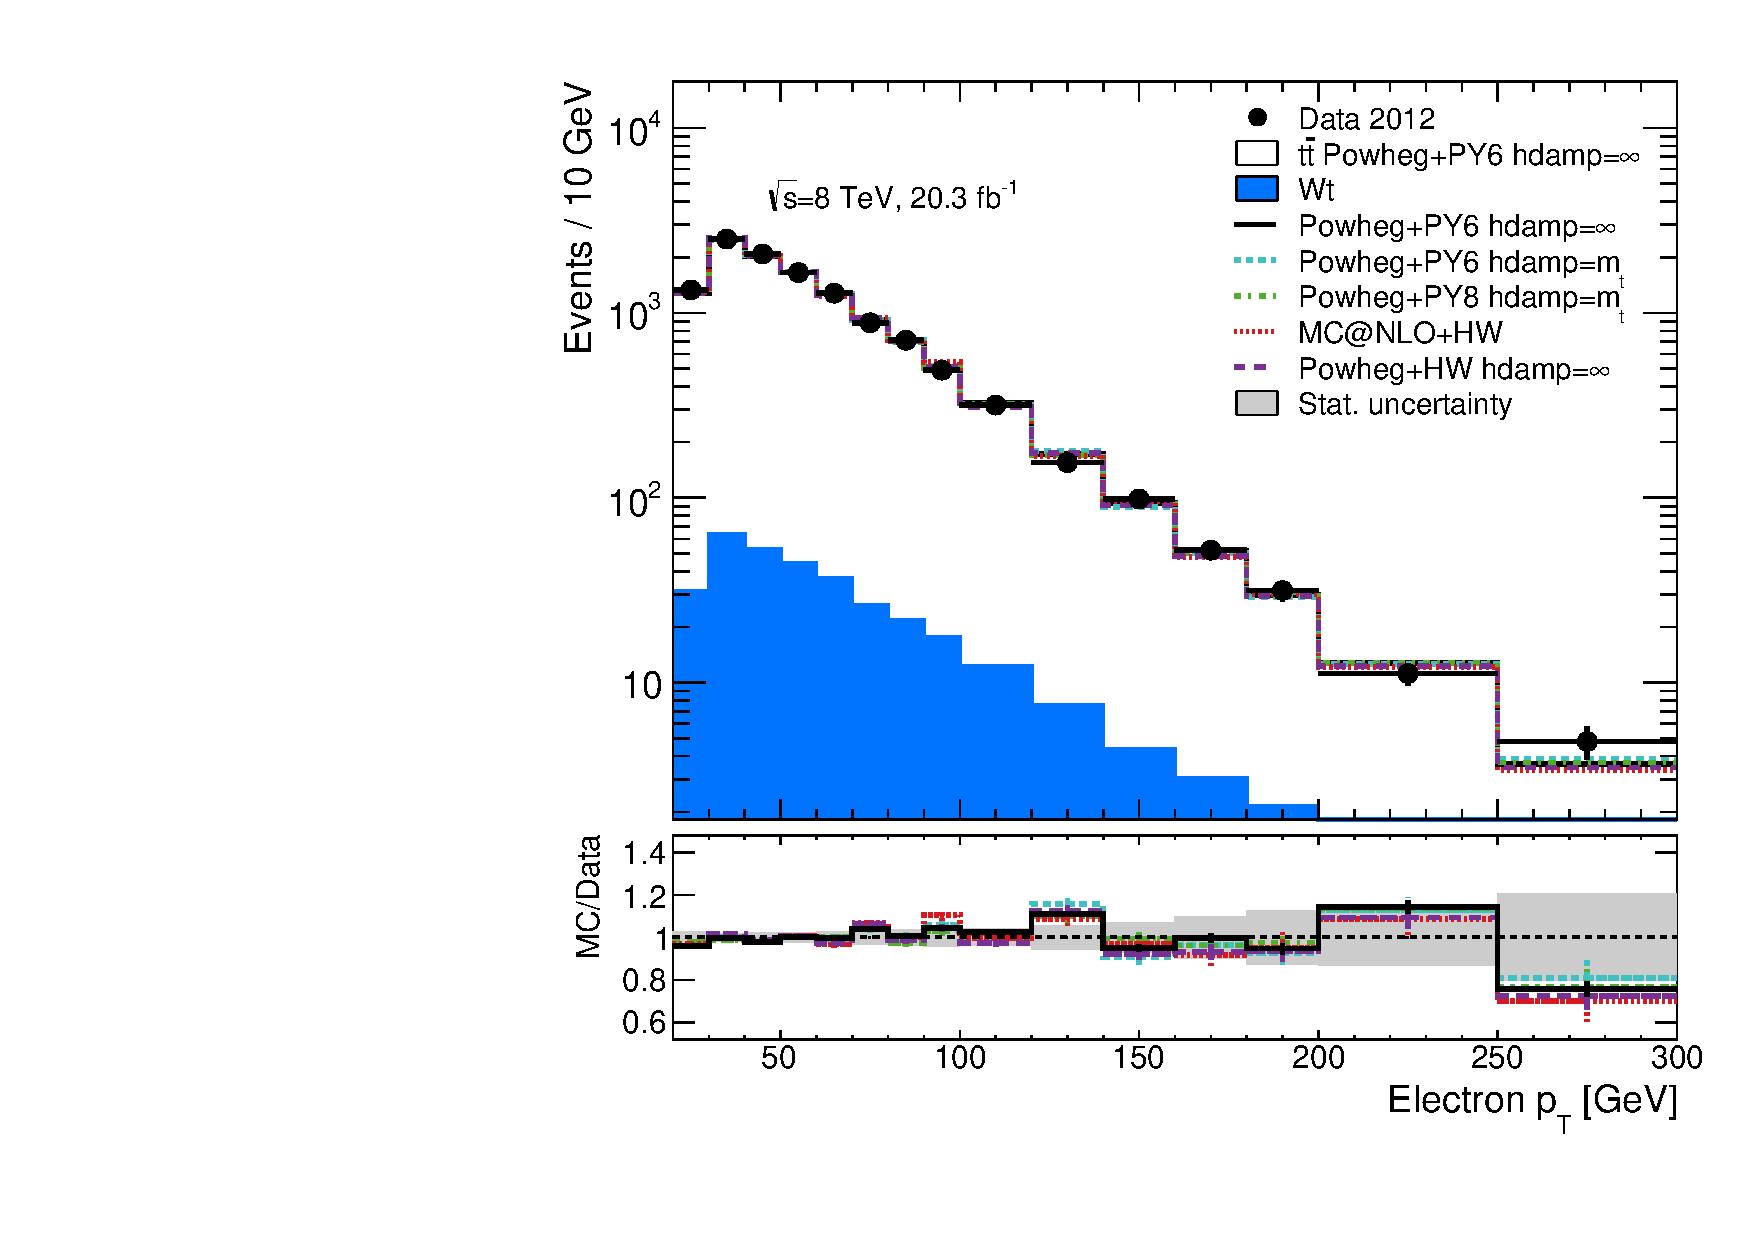
\includegraphics[width=0.45\textwidth]{fig/MCComp/NLO/ElecPt.pdf}}
\subfloat[]{
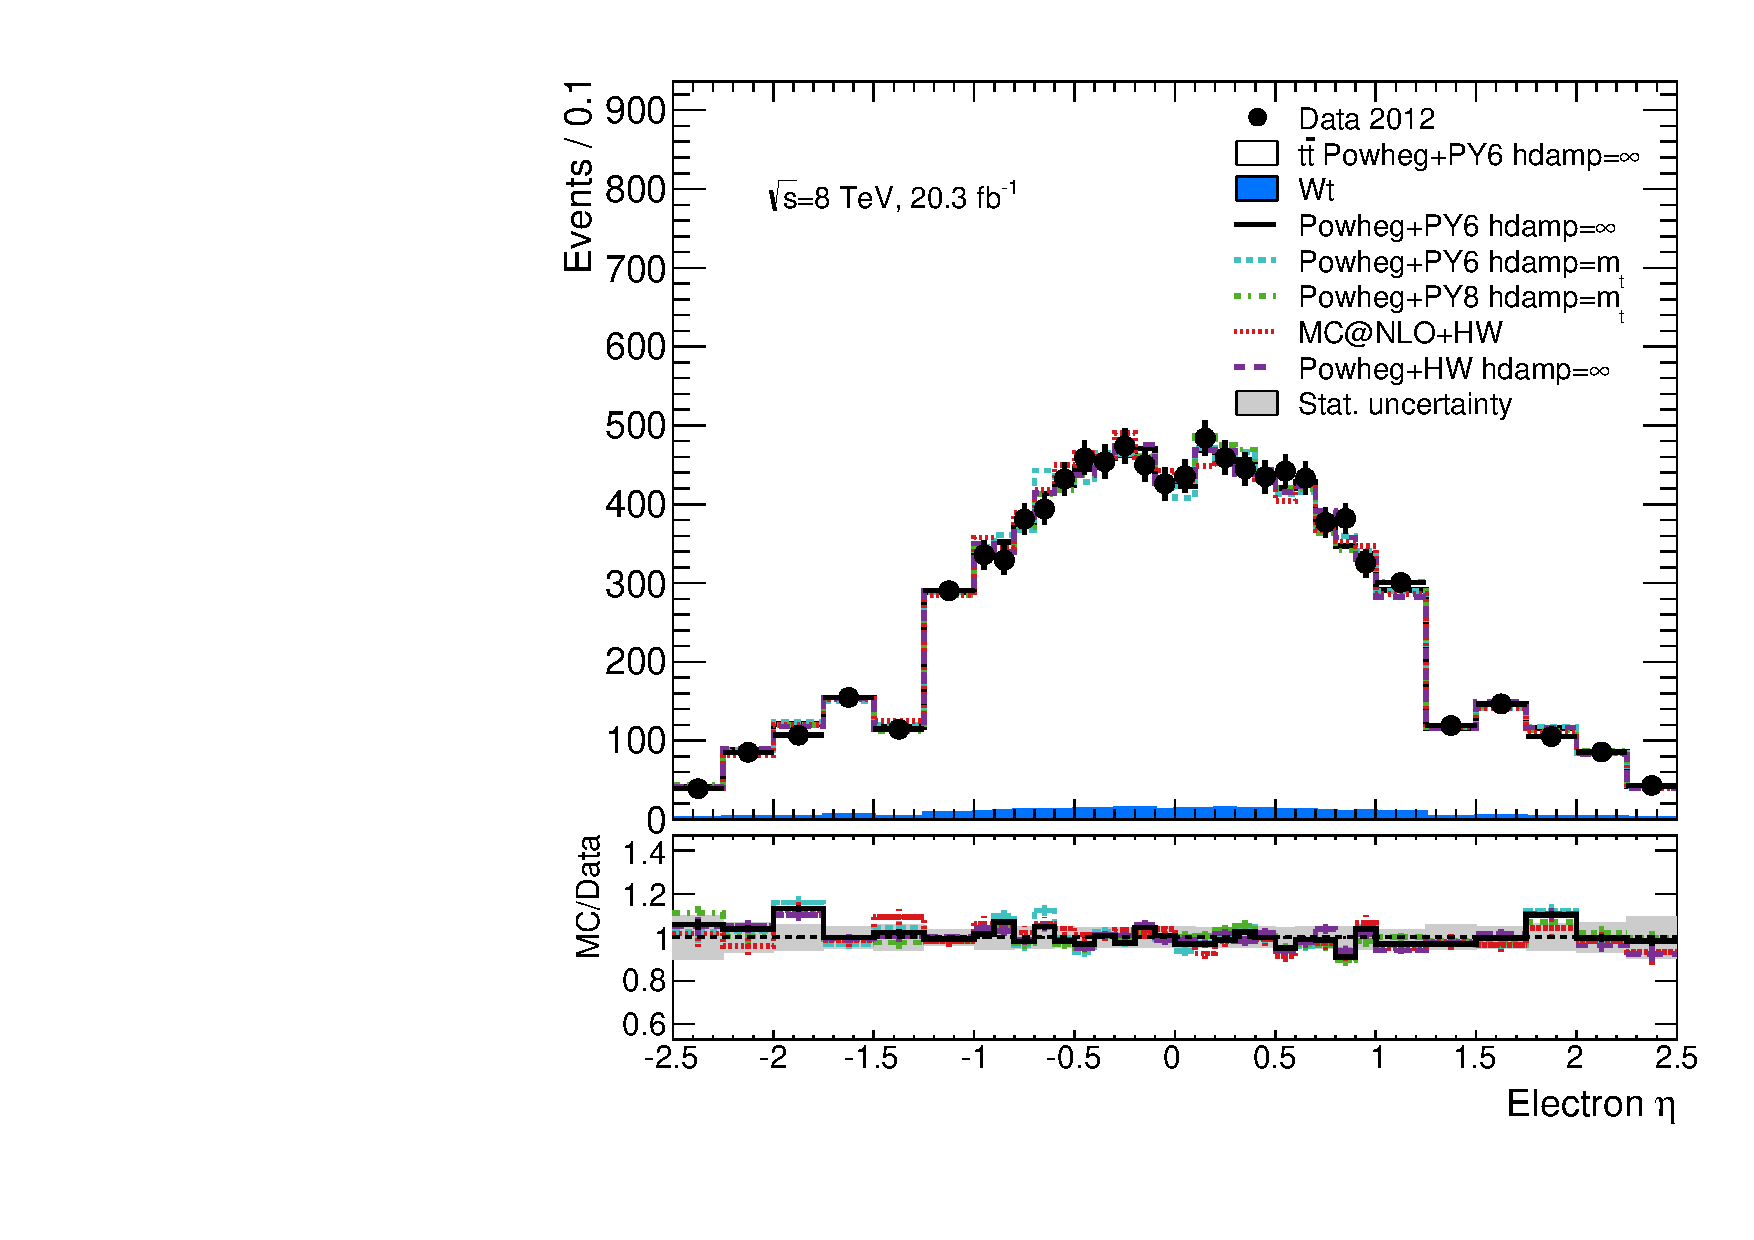
\includegraphics[width=0.45\textwidth]{fig/MCComp/NLO/ElecEta.pdf}}
\\
\subfloat[]{
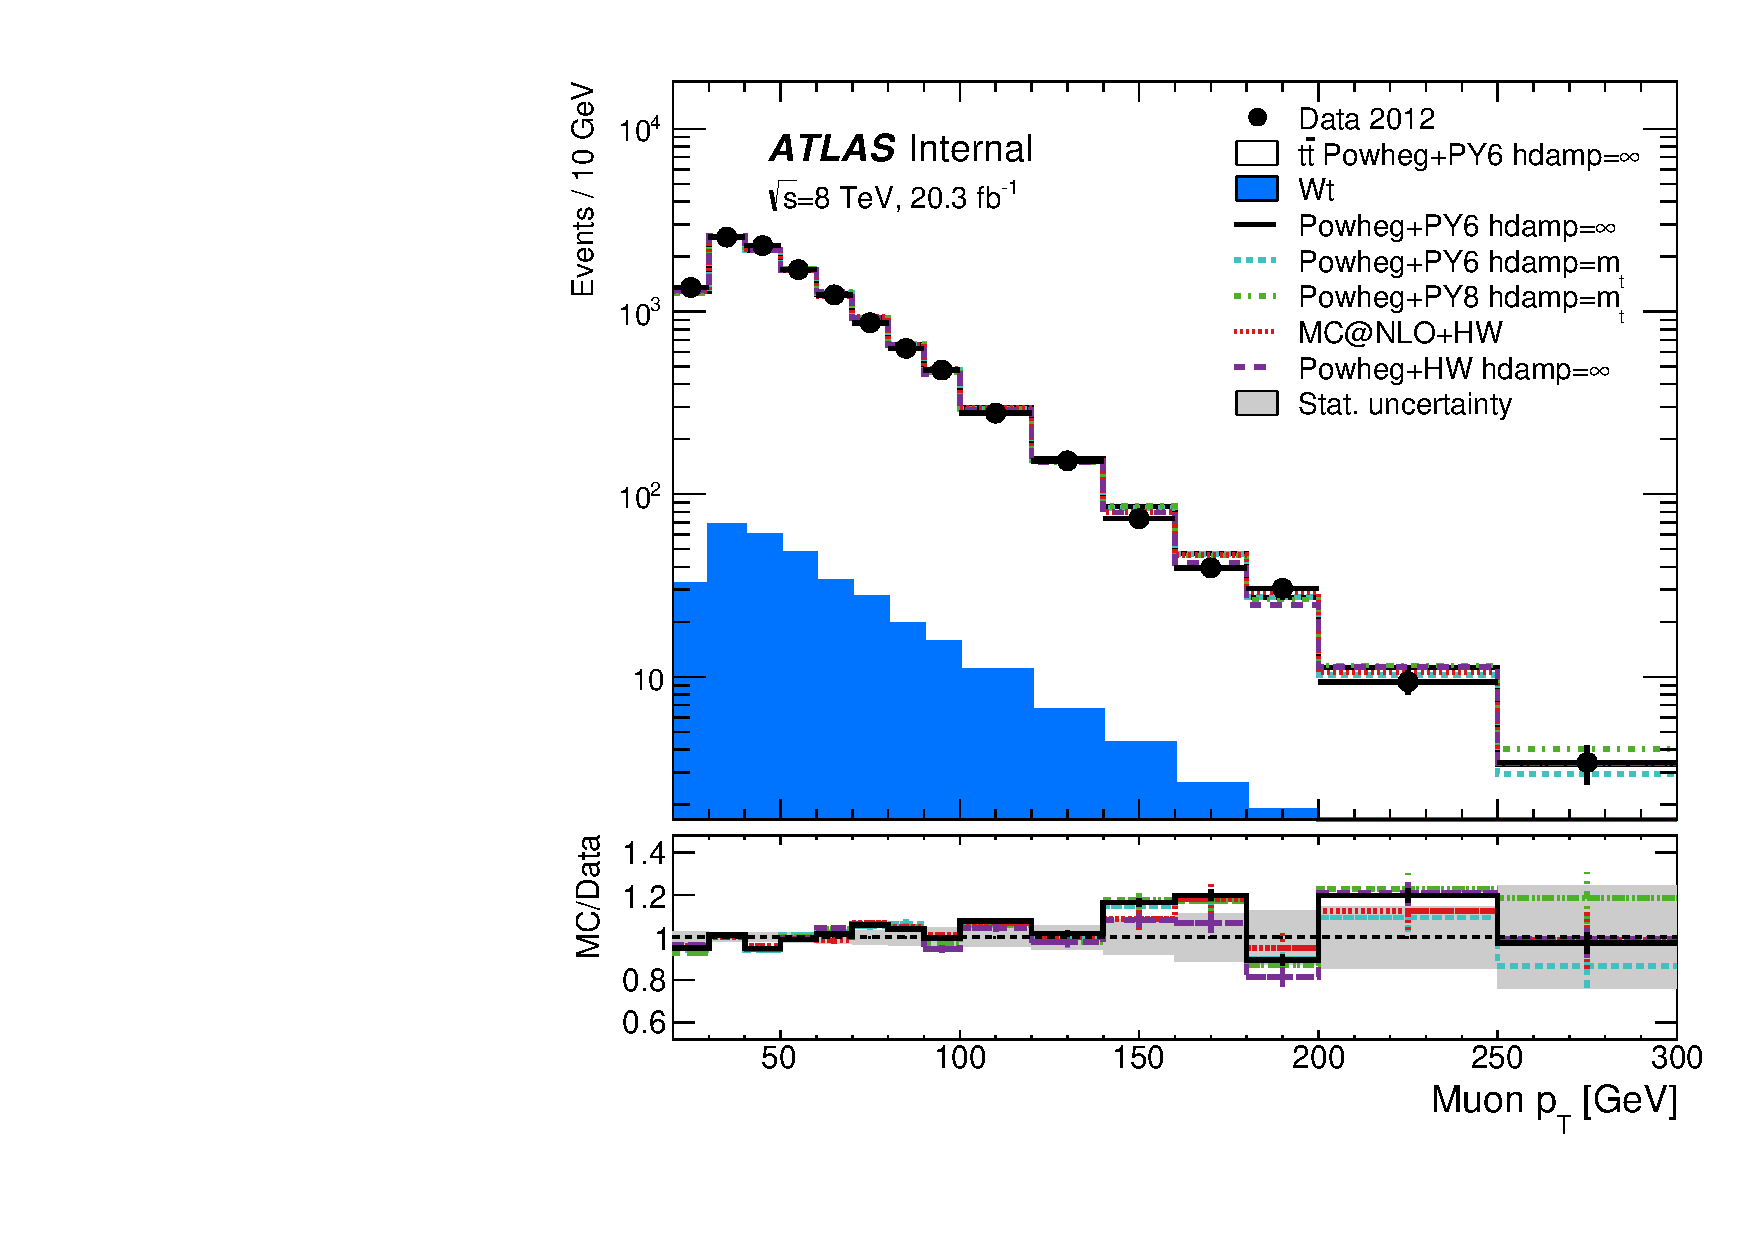
\includegraphics[width=0.45\textwidth]{fig/MCComp/NLO/MuPt.pdf}}
\subfloat[]{
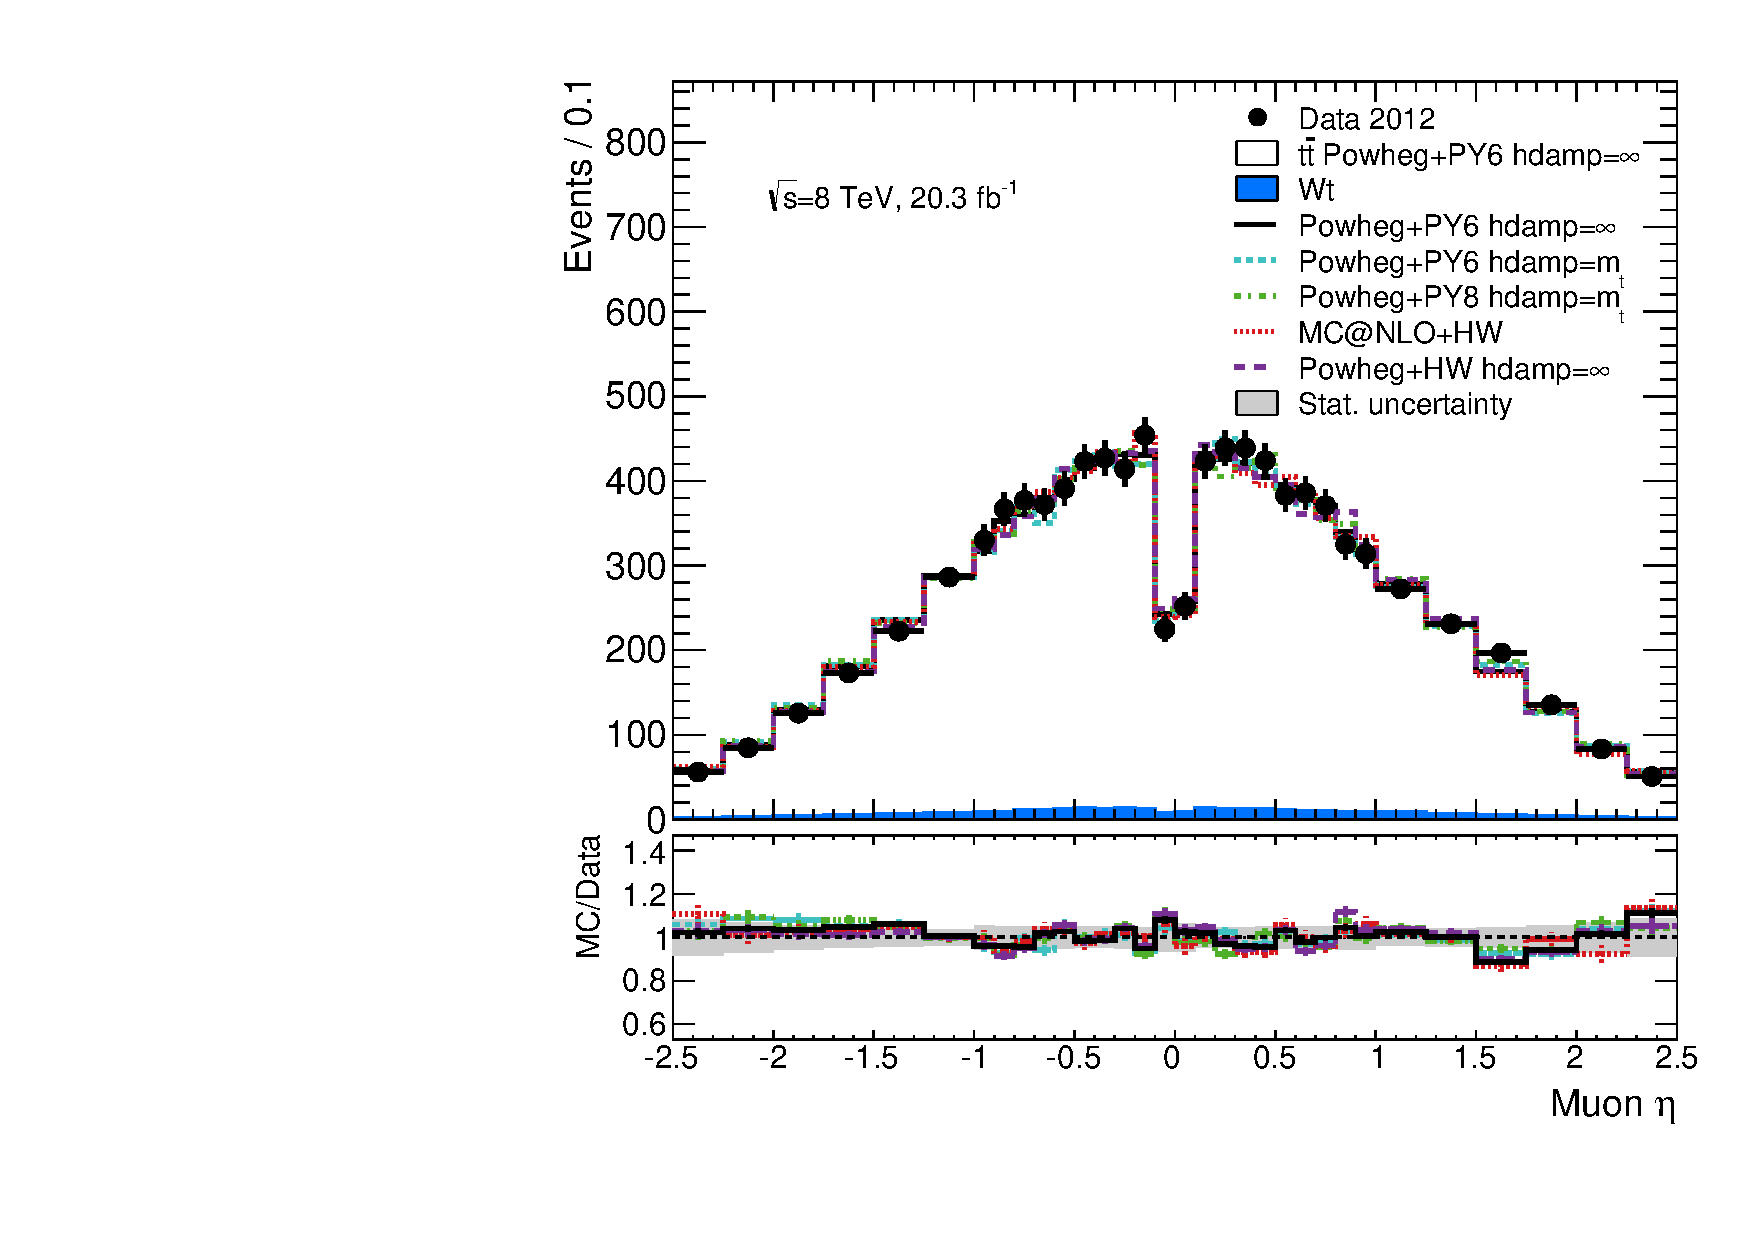
\includegraphics[width=0.45\textwidth]{fig/MCComp/NLO/MuEta.pdf}}
\caption{Distributions of the transverse momentum and $\eta$ of the electron and muon in events with an opposite sign $e\mu$ pair and at least 2 $b$-jets in data and simulation. The distributions in data are compared to simulation normalized to data yields (see scale factors in Table~\ref{t:ttgen}). The ratio of different MC samples to data is shown with error bars corresponding to the MC statistical uncertainty and a shaded band corresponding to the data statistical uncertainty.}
\label{fig:emu}
\end{figure}

\begin{figure}
\centering
\subfloat[]{
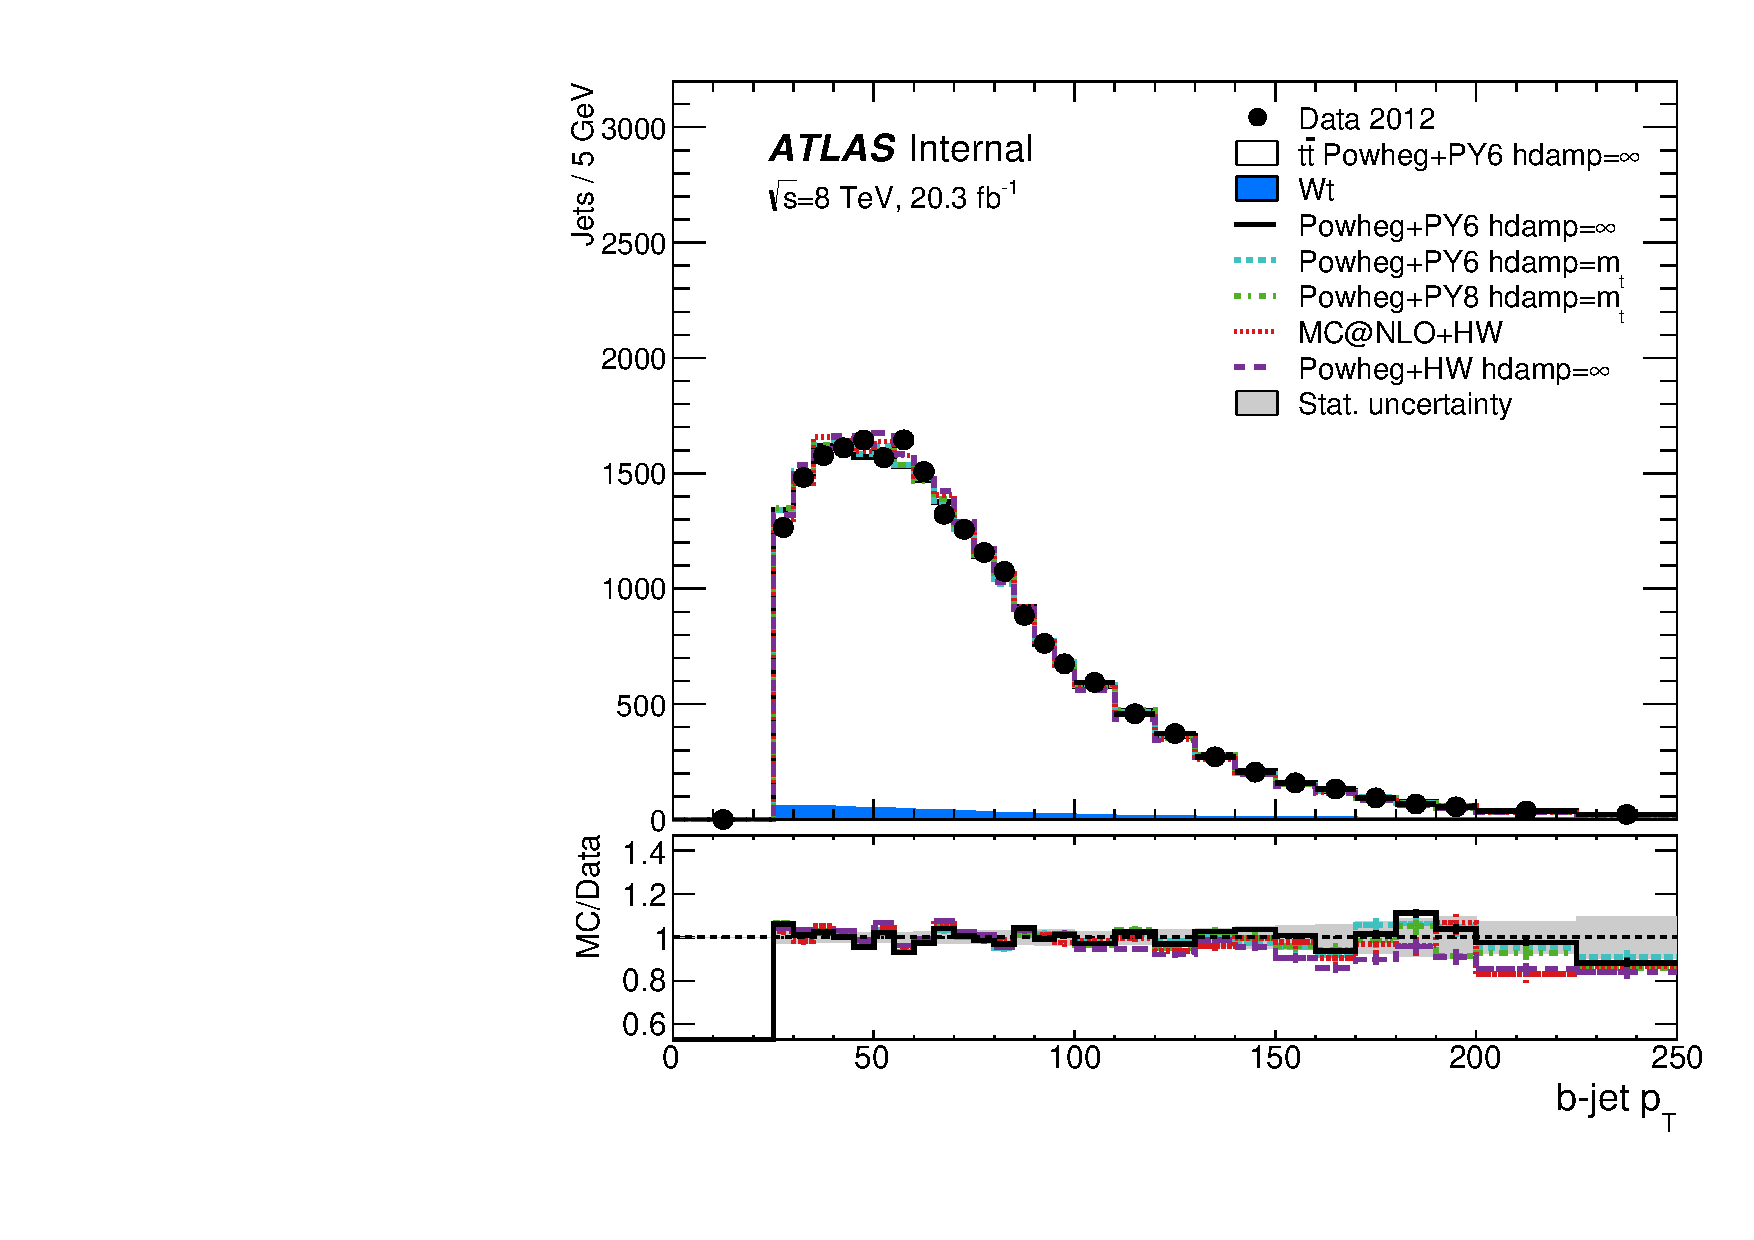
\includegraphics[width=0.45\textwidth]{fig/MCComp/NLO/BJetPt.pdf}}
\subfloat[]{
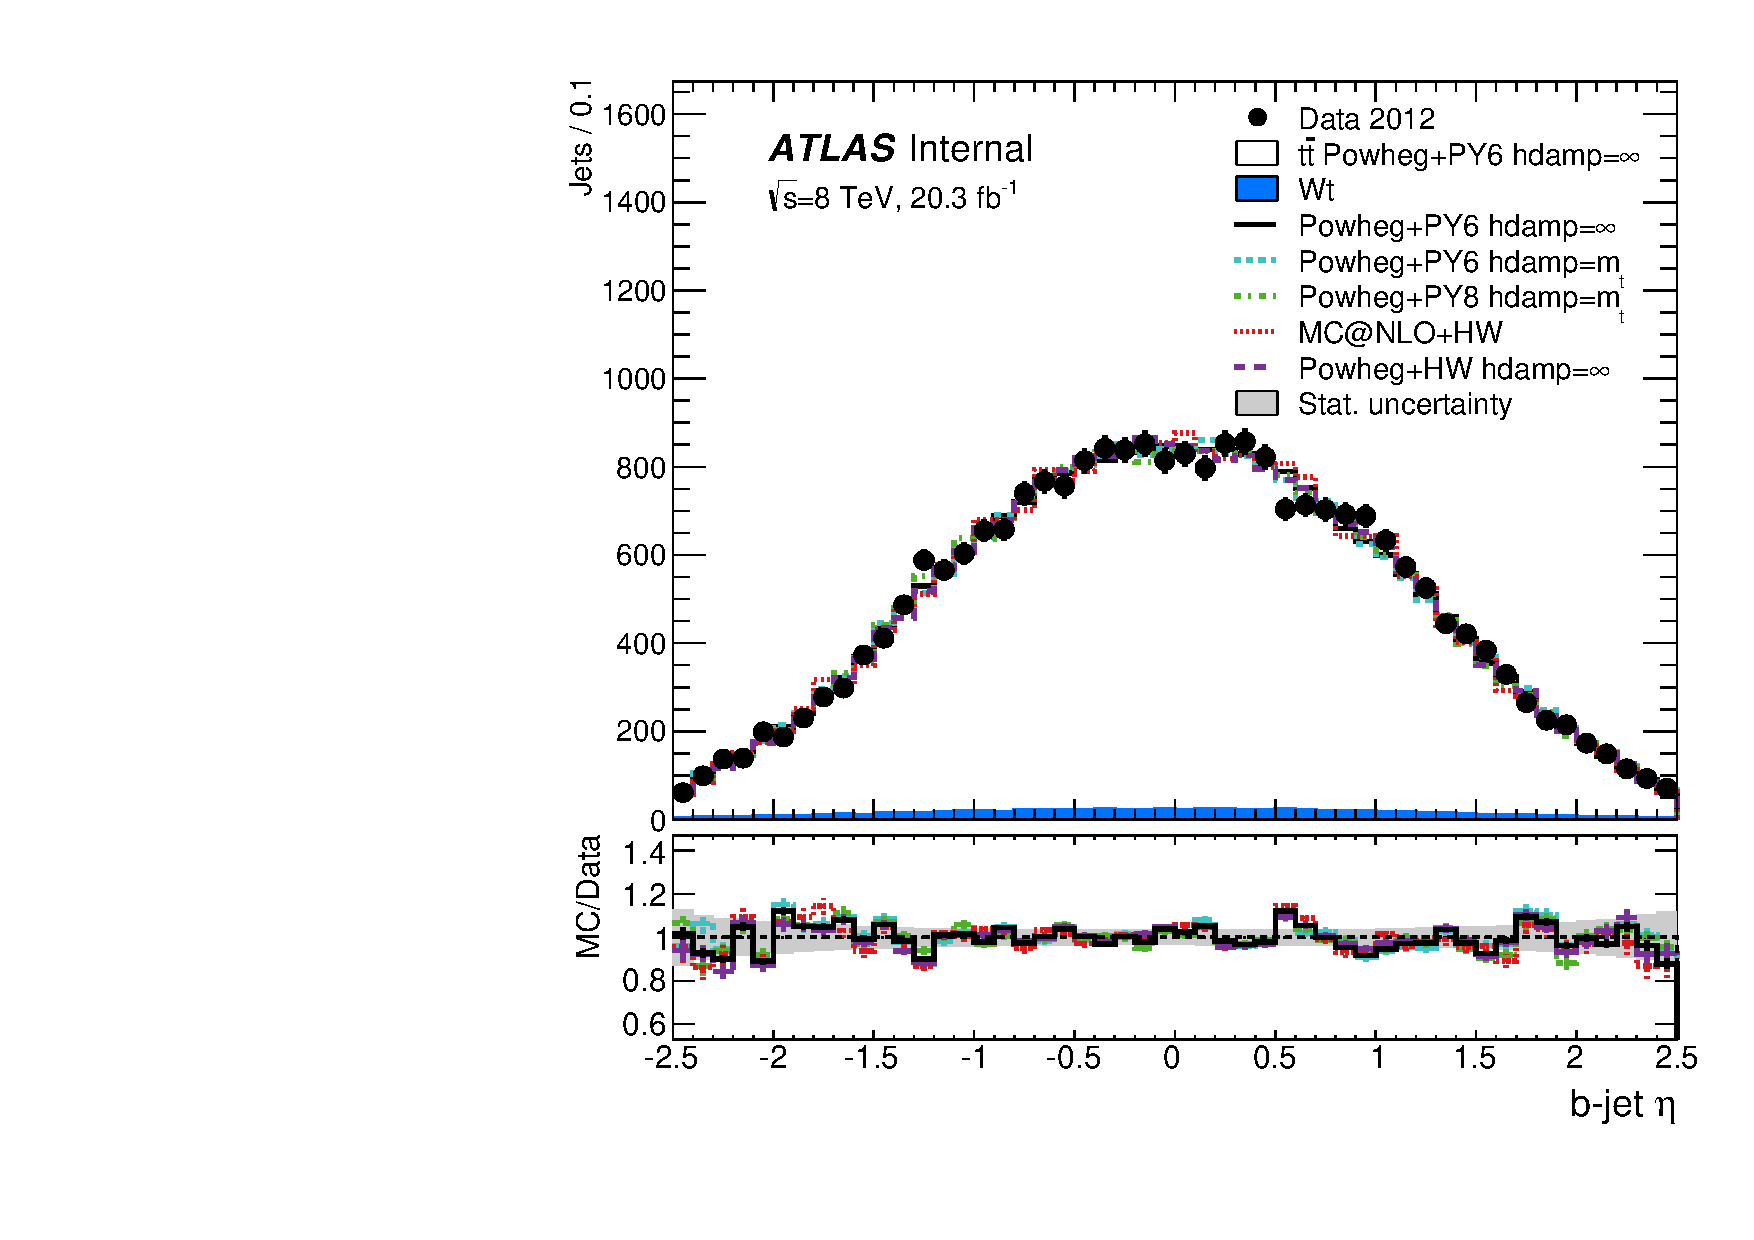
\includegraphics[width=0.45\textwidth]{fig/MCComp/NLO/BJetEta.pdf}}

\caption{Distributions of the transverse momentum and $\eta$ of the $b$-jets in events with an opposite sign $e\mu$ pair  and at least 2 $b$-jets in the 2012 data. The distributions in data are compared to simulation, normalized to the same number of events as in the data  (see scale factors in Table~\ref{t:ttgen}).. In events where more than two $b$-jets are reconstructed, the two highest \pt $b$-jets are selected and the remaining $b$-jet is classified as an extra jet (see Section ~\ref{sec:extrajets}). The ratio of different MC samples to data are shown with error bars corresponding to the MC statistical uncertainty and a shaded band corresponding to the data statistical uncertainty. Systematic uncertainties are not shown.}
\label{fig:bjet}
\end{figure}

